\section{Optimization for Sparse Convex Additive Models}

We now consider the following nonparametric regression problem
\begin{equation}\nonumber
          Y_{i} = f(\bds{x}_{i}) + \epsilon_{i} = 
                  \sum_{k=1}^{p}f_{k}(x_{ki}) + \epsilon_{i} \quad i=1,2,\cdots,n
\end{equation}
where $\bds{x}_{i}\in\mathbb{R}^{p}$ is the covariate, $Y_{i}$ is the
response and $\epsilon_{i}$ is mean zero noise. The regression function $f(\cdot)$ is the summation of 
functions $f_{k}(\cdot)$ in each variable dimension.  
We impose an additional constraint that each $f_{k}(\cdot)$ is 
a univariate convex function, which can be represented by its supporting hyperplanes, i.e.,
\begin{equation}\label{hyper}
      h_{kj} \geq h_{ki} + \beta_{ki}(x_{kj}-x_{ki}) \quad (\forall i,j)
\end{equation}
where $h_{ki}\coloneqq f_{k}(x_{ki})$ and $\beta_{ki}$ is the
subgradient at point $x_{ki}$. We apparently need $O(n^2 p)$ constraints to
impose the supporting hyperplane constraints, which is computationally
expensive for large scale problems.  In fact, only $O(np)$
constraints suffice, since univariate convex functions are
characterized by the condition that the subgradient, which is a scalar, must
increase monotonically. This observation leads to our optimization
program:
\begin{equation}
\begin{split}
       \min_{\bds{h},\bds{\beta},\mu} & \;\; \frac{1}{2n}\sum_{i=1}^{n}
                     \Bigl( Y_{i}-\sum_{k=1}^{p}h_{ki} - \mu \Bigr)^{2} 
                         + \lambda\sum_{k=1}^{p}\|\bds{\beta}_{k\cdot}\|_{\infty} \\
       \textrm{subject to} &\;\; h_{k(i+1)} = h_{k(i)} + \beta_{k(i)}(x_{k(i+1)}-x_{k(i)}), \\
                     & \;\; \sum_{i=1}^{n}h_{ki}=0,\\
                     & \;\; \beta_{k(i+1)} \geq \beta_{k(i)} \ (\forall k, i)
\end{split}
\label{np}
\end{equation}
Here $\{(1),(2),\ldots,(n)\}$ is a reordering of $\{1,2,\ldots,n\}$ such that $x_{k(1)}\leq{}x_{k(2)}\leq\cdots\leq{}x_{k(n)}$.  We introduce a mean parameter $\mu \in \R$ because $f$ may not have
zero mean. We can in fact solve for $\mu$ explicitly, as  
$\mu = \frac{1}{n} \sum_{i=1}^n Y_i = \bar{Y}$ which follows from the
KKT conditions
and the constraints $\sum_i h_{ki} = 0$.
It is easy to verify that the constraints in (\ref{np}) satisfy the supporting hyperplane constraints, as
\begin{align*}
  \forall j\geq{}i, &h_{k(j)}-h_{k(i)}  = 
            \sum\limits_{t=i}^{j-1}(h_{k(t+1)}-h_{k(t)}) = 
            \sum\limits_{t=i}^{j-1}\beta_{k(t)}(x_{k(t+1)}-x_{k(t)})\\ 
      & \geq \beta_{k(i)}\sum\limits_{t=i}^{j-1}(x_{k(t+1)}-x_{k(t)}) = \beta_{k(i)}(x_{k(j)}-x_{k(i)}) \\
  \forall j<i, &h_{k(j)}-h_{k(i)} =
                \sum\limits_{t=j}^{i-1}(h_{k(t)}-h_{k(t+1)}) = 
                \sum\limits_{t=j}^{i-1}\beta_{k(t)}(x_{k(t)}-x_{k(t+1)}) \\ 
     & \geq \beta_{k(i)}\sum\limits_{t=j}^{i-1}(x_{k(t)}-x_{k(t+1)}) = \beta_{k(i)}(x_{k(j)}-x_{k(i)}), 
\end{align*}
The $\ell_\infty/\ell_1$ penalty
$\sum_{k=1}^{p}\|\bds{\beta}_{k\cdot}\|_{\infty}$ encourages group
sparsity of the vectors $\bds{\beta}_{k\cdot}$, and thus performs
variable selection.  We refer to this framework as the sparse convex
additive model (SCAM). While one can use
supporting hyperplanes to the epigraph as in \eqref{eq:outer}, 
SCAM uses the \emph{inner  piece-wise linear function}
that approximates the graph with secant lines. Notice that if we replace $\beta_{k(i+1)} \geq
\beta_{k(i)}$ with $\beta_{k(i+1)}=\beta_{k(i)}$, the optimization
reduces to the lasso.  


%\begin{SCfigure}
%\label{fig:outer_approximation}
%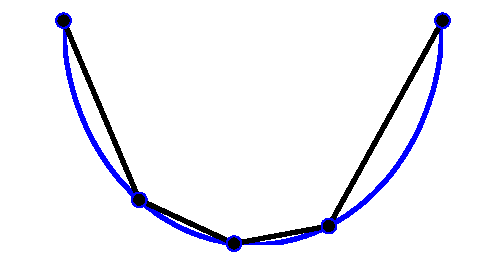
\includegraphics[width=0.3\textwidth]{figs/outer_approximation.pdf}
%\caption{With the 5 sample points $(X_i, h(X_i))$, the
%  black and the blue convex function represent equivalent fits. SCAM
%  chooses the inner piece-wise linear convex functions.}
%\end{SCfigure}

The SCAM optimization in (\ref{np}) is a quadratic program (QP) with $O(np)$ variables and $O(np)$ constraints. The optimal $\mu$ has a closed form solution of $\mu = \frac{1}{n}\sum_{i=1}^n Y_i$, which is easy to derive from the KKT theorem and the constraints that $\sum_i h_{ki} = 0$ for all $k$.
Directly applying a QP solver for $\bds{h}, \bds{\beta}$ would be computationally expensive for relatively large $n$ and $p$. However, notice that variables
in different feature dimensions are only coupled in the term $(Y_{i}-\sum_{k=1}^{p}h_{ki})^{2}$. Hence, we can apply the block coordinate descent method,
where in each step we solve the following QP subproblem for
$\{\bds{h}_{k\cdot},\bds{\beta}_{k\cdot}\}$ with the other variables fixed:
\begin{equation}\begin{split}\nonumber
       &\min_{\bds{h}_{k\cdot},\bds{\beta}_{k\cdot},\gamma_{k}} 
             \ \frac{1}{2n}\sum_{i=1}^{n}\Bigl((Y_{i}-\bar{Y}-\sum_{r\neq{k}}h_{ri})-h_{ki}\Bigr)^{2} 
                      + \lambda\gamma_{k} \\
        &\ \textrm{s.t.} \ \sum_{i=1}^{n}h_{ki}=0, \ h_{k(i+1)} = h_{k(i)} + \beta_{k(i)}(x_{k(i+1)}-x_{k(i)}), \ \beta_{k(i+1)} \geq \beta_{k(i)}, \ -\gamma_{k}\leq\beta_{k(i)}\leq\gamma_{k} \ (\forall i).
\end{split}\end{equation}
The extra variable $\gamma_{k}$ is introduced to deal with the $\ell_{\infty}$ norm. This QP subproblem involves $O(n)$ variables, $O(n)$ constraints and a sparse structure, 
which can be solved efficiently using optimization packages (e.g., MOSEK: \verb+http://www.mosek.com/+).  We cycle through all feature dimensions ($k$) from $1$ to $p$ multiple times until convergence.
Empirically, we observe that the algorithm converges in only a few cycles. We also implemented an ADMM solver for (\ref{np}), but found that it is not as efficient as this QP solver.

After optimization, the function estimator for any input data $\bds{x}_j$ is, according to (\ref{hyper}),
\begin{equation}\nonumber
      f(\bds{x}_j) = \sum_{k=1}^{p}f_k(x_{kj})+\mu = \sum_{k=1}^{p}\max_{i} \{h_{ki}+\beta_{ki}(x_{kj}-x_{ki})\} + \mu.
\end{equation} 


\subsection{Alternative Formulation}
Optimization (\ref{np}) can be reformulated in terms of the 2nd derivatives. The alternative formulation replaces the ordering
constraints $\beta_{k(i+1)} \geq \beta_{k(i)}$ with positivity
constraints, which simplifies theoretical analysis.
Define $d_{k(i)}$ as the second derivative:
$d_{k(1)} = \beta_{k(1)}$, and $d_{k(2)} =
\beta_{k(2)} - \beta_{k(1)}$. The convexity constraint is
equivalent to the constraint that $d_{k(i)} \geq 0$ for all $i >
1$.

It is easy to verify that $\beta_{k(i)} = \sum_{j \leq i} d_{k(i)}$ and 
\[
f_k(x_{k(i)}) = f_k({x_{k(1)}}) +d_{k(1)} ( x_{k(i)}
- x_{k(1)}) + d_{k(2)} ( x_{k(i)} - x_{k(2)}) + \cdots + d_{k(i-1)} ( x_{k(i)} - x_{k(i-1)})
\]
We can write this more compactly in matrix notations. First define $\Delta_{k(j)}(x_{ki}) = \max( x_{ki} - x_{k(j)}, 0)$. 
\[
\left[ \begin{array}{c}
    f_k(x_{k1}) \\
    ... \\
    f_k(x_{kn}) \\
\end{array} \right] =
\left[ \begin{array}{ccc}
    \Delta_{k(1)}(x_{k1}) & ... & \Delta_{k(n-1)}(x_{k1}) \\
    ... & & \\
    \Delta_{k(1)}(x_{kn}) & ... & \Delta_{k(n-1)}(x_{kn}) 
\end{array} \right]
\left[ \begin{array}{c}
    d_{k(1)} \\
    ... \\
    d_{k(n-1)}
\end{array} \right] \coloneqq \Delta_k d_k
\]
Where $\Delta_k$ is a $n\times n-1$ matrix such that $\Delta_k(i,j) = \Delta_{k(j)}(x_{k(i)})$ and $d_k = (d_{k(1)} ,..., d_{k(n-1)})$. We can now reformulate (\ref{np}) as an equivalent optimization program with only centering and positivity constraints:
\begin{align}
\min_{d_k \in \R^{n-1}, c_k \in \R,\mu \in \R}& \frac{1}{2n} 
       \Bigl\| Y - \bar{Y}\mathbf{1}_n - \sum_{k=1}^p ( \Delta_k d_k - c_k \mathbf{1}_n) \Bigr\|_2^2 
               + \lambda_n \sum_{k=1}^p \|d_k\|_1  & \label{opt:alternate_opt} \\
\trm{s.t. $\forall k$, }  & d_{k(2)}, \ldots , d_{k(n-1)} \geq 0 	
               \qquad &\trm{(convexity)} \nonumber \\ 
	& c_k = \frac{1}{n} \mathbf{1}_n^\tran \Delta_k d_k 	
               \qquad &\trm{(centering)} \nonumber 
\end{align}
$\|d_k\|_1$ is not identical to $\|\bds{\beta}_{k\cdot}\|_{\infty}$, but it is easy to verify that $\|\bds{\beta}_{k\cdot}\|_{\infty} \leq \|d_k\|_1 \leq 2\|\bds{\beta}_{k\cdot}\|_{\infty}$.

\begin{remark}
\label{rem:bounded_lipschitz_constraints}
For parts of our theoretical analysis, we will also impose onto (\ref{opt:alternate_opt}) a boundedness constraint $-B \mathbf{1}_n \leq \Delta_k d_k + c_k \mathbf{1}_n \leq B \mathbf{1}_n$ which constrains that $\|f_k \|_\infty \leq B$, or a Lipschitz constraint $\|d_k\|_1 \leq L$ which constrains that $f_k$ must be $L$-Lipschitz. We use these constraints only in the proof for technical reasons; we never need nor use these constraints in our experiments.
\end{remark}


